\documentclass[12pt]{report}
\usepackage{geometry}
\usepackage{graphicx}
\usepackage{xcolor}
\usepackage{titlesec}
\usepackage{float} 
\usepackage{url}

\setcounter{secnumdepth}{4}
\graphicspath{ {./images/} }

\begin{document}

	
	\tableofcontents
	\listoffigures
	\listoftables
	
	
	\chapter{Generality}
	\section{Internet of Things Technology (IoT) }
	\subsection{Definition}
	
IoT, or Internet of Things, is a system of interconnected physical devices, vehicles, buildings, and other objects that have been embedded with sensors, software, and network connectivity to collect and exchange data.
IoT technology provides real-time data for monitoring and controlling processes and functions, with potential to revolutionize industries like manufacturing, healthcare, transportation, and energy.
The implementation of IoT poses challenges such as heterogeneity, complexity, poor interoperability, resource constraints, and privacy concerns, which must be addressed to fully realize the benefits of this technology.\cite{dai2019blockchain}
	\begin{figure}[H]
	\centering
	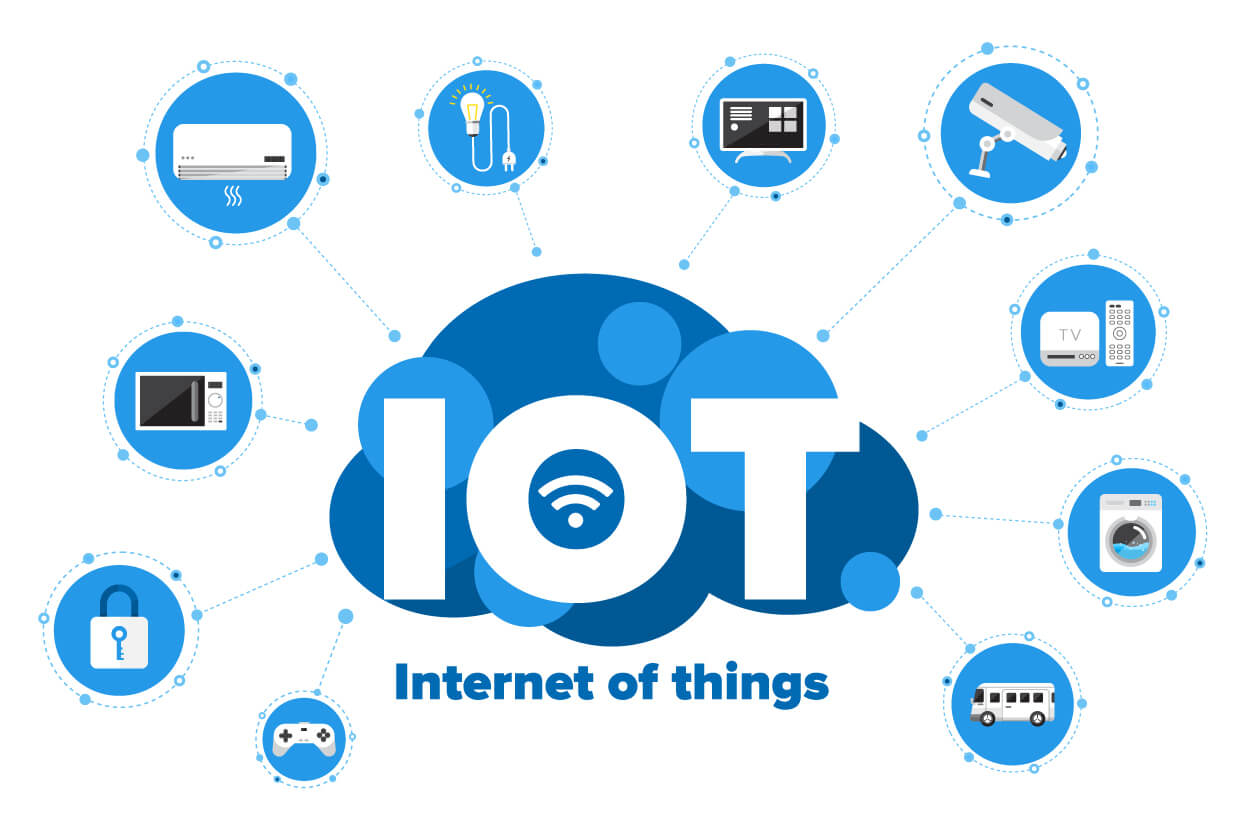
\includegraphics[width=0.5\textwidth]{iot.jpg}
	\caption{A sample image of IoT devices\cite{globalsign-iot}.}
	\label{fig:iot}
\end{figure}

	\subsection{Architectures}
	The Internet of Things (IoT) is a technology that includes three main layers the Perception Layer, Transmission Layer and Application Layer.\cite{gupta2020overview}
		\begin{figure}[H]
		\centering
		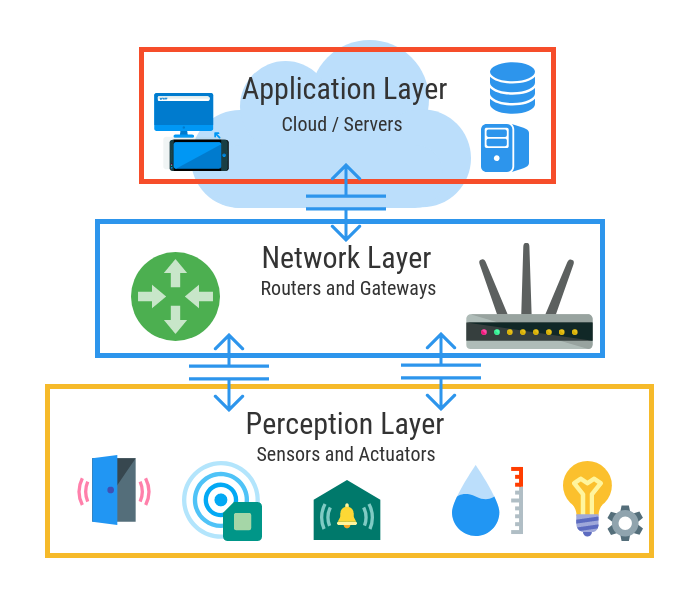
\includegraphics[width=0.6\textwidth]{three-layer-iot-architecture}
		\caption{The fundamental Three Layer IoT Architecture
			\cite{netburner}.}
		\label{fig:3layers}
	\end{figure}
	\subsubsection{Perception Layer}
	
The Perception Layer is the lowest layer in the IoT architecture, sometimes called the Device, Sensory, or Recognition Layer. It is responsible for sensing, identifying, and communicating with the physical world in a digital format. This layer captures data with little human intervention.
The Perception Layer of the IoT architecture consists of the Perception Nodes and the Perception Network.
	\subsubsection*{Perception Nodes}
	The Perception Nodes refer to the physical devices such as sensors, actuators, and controllers that form a network to collect data and control objects. This network can be established through various technologies, including RFID readers, QR code or Barcode readers, GPS devices, Bluetooth devices, and various sensors. The Perception Nodes identify objects, collect data from the environment, and control objects. 
	\subsubsection*{Perception Networks}
The Perception Network communicates with the Transmission Network, securely transmitting data collected by the Perception Nodes to gateways for further transmission and sending control signals to controller devices through wired or wireless communication mediums.
	\subsubsection{Transmission (Network) Layer}
	The Transmission Layer is an important part of the IoT architecture that sits between the Perception and Application Layers. It's responsible for integrating various networks, technologies, and protocols to transmit data from Perception Nodes to higher level decision-making units. The data is transferred through wired or wireless communication channels, and the layer provides functionalities for network management. The Transmission Layer is also responsible for providing necessary support for analyzing, encoding, aggregating and data mining. It can be divided into three sub-layers below :
	\begin{itemize}
		\item Access Network
		\item Core Network
		\item Local and Wide Area Network
	\end{itemize}
	\begin{figure}[H]
	\centering
	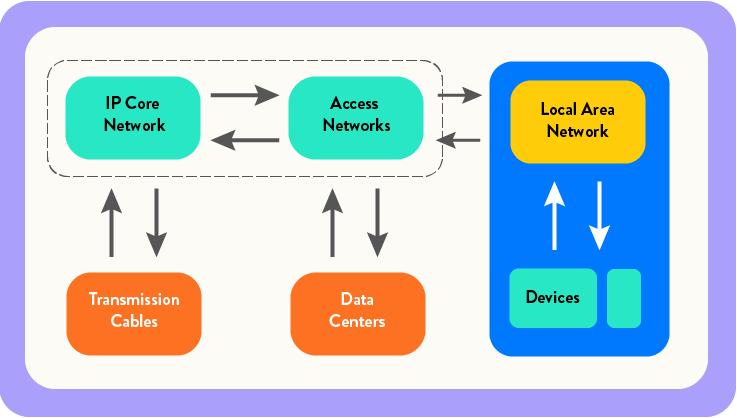
\includegraphics[width=0.8\textwidth]{network}
	\caption{illustration showing a network system diagram
		\cite{sustainablewebdesign}.}
	\label{fig:networklayer}
\end{figure}
	\subsubsection{Application Layer}
	The Application Layer is the highest layer of the IoT architecture, visible to the end user. Its purpose is to manage and provide applications globally based on the information collected by the Perception Layer, which is processed by the Information Processing Unit. This layer provides access to personalized services for end-users over the network through the use of various handheld devices and terminal equipment. It can be divided into two sub-layers: Application Support Layer and IoT Applications.\\
	 The Application Support Layer is located just above the Transmission Layer, responsible for performing intelligent computations and processing over data. It performs data recognition and filtration to categorize it as valid or invalid, and utilizes middleware, Cloud Computing, and Service Support Platform to provide support services for the applications
	
	\subsection{Protocoles}
	IoT protocols are a set of rules that allow electronic devices to exchange and transmit data with each other and the internet. These protocols can be classified into two categories: IoT network protocols and IoT data protocols. Network protocols help connect IoT devices with other edge devices or the internet, while data protocols focus on exchanging information, each category has its own set of protocols that come with unique features, which we will examine in the following section.\cite{particleIoT}
	\begin{figure}[H]
		\centering
		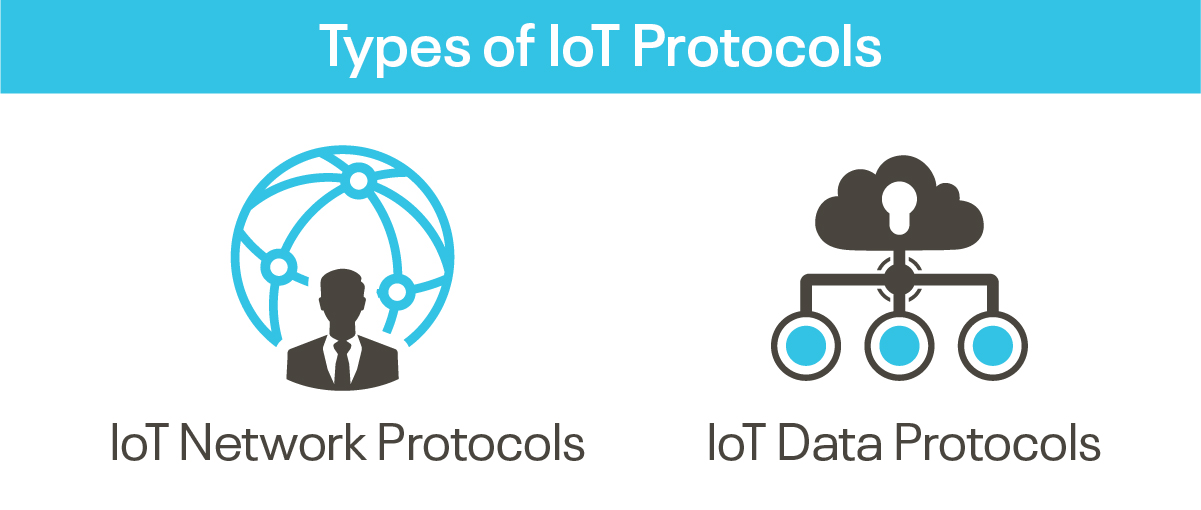
\includegraphics[width=1\textwidth]{iot-protocoles}
		\caption{IoT Protocols
			\cite{netburner}.}
		\label{fig:2protocoles}
	\end{figure}
	\subsubsection{IoT Network Protocols}
	\begin{figure}[H]
	\centering
	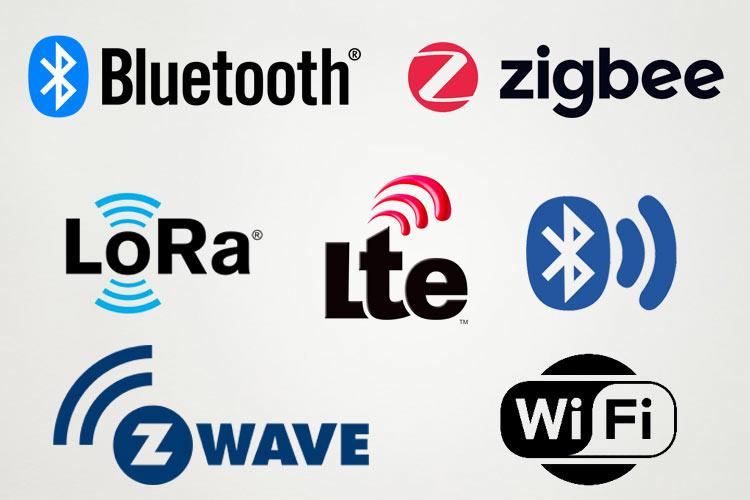
\includegraphics[width=0.7\textwidth]{network-protocol}
	\caption{The IoT Network Protocols
		\cite{iotdesignpro}.}
	\label{fig:NetworkProtocols}
\end{figure}
	\subsubsection*{Wi-Fi}
	Wi-Fi, defined by the IEEE 802.11 standard, is a widely used wireless LAN protocol for transmitting large volumes of data over reasonable distances. Low-power IoT devices avoid it due to high power consumption.
	\subsubsection*{Bluetooth}
	Bluetooth is a short-range wireless technology standard for exchanging data between devices over short distances. It's used in IoT to connect small, battery-powered sensors to gateways or other smart devices. With limited transmission power of 2.5 milliwatts, it has a short range of up to 10 metres.
	\subsubsection*{ZigBee}
	ZigBee is a wireless network technology used in home or building automation settings. It's low-cost, low-power and reliable, and supports multiple network topologies. ZigBee devices combine application, logical, and physical types. The standard was ratified in the early 2000s.\cite{inproceedings}
	\subsubsection*{LoRaWAN}
	The LoRaWAN is a Low Power, Wide Area (LPWA) protocol designed to attach battery-powered gadgets to the net in regional, countrywide or international networks. It addresses key IoT requirements like secure two-way communication, mobility, and localization services.\cite{lorawanSpec}
	\subsubsection {IoT Data Protocols}
		\begin{figure}[H]
		\centering
		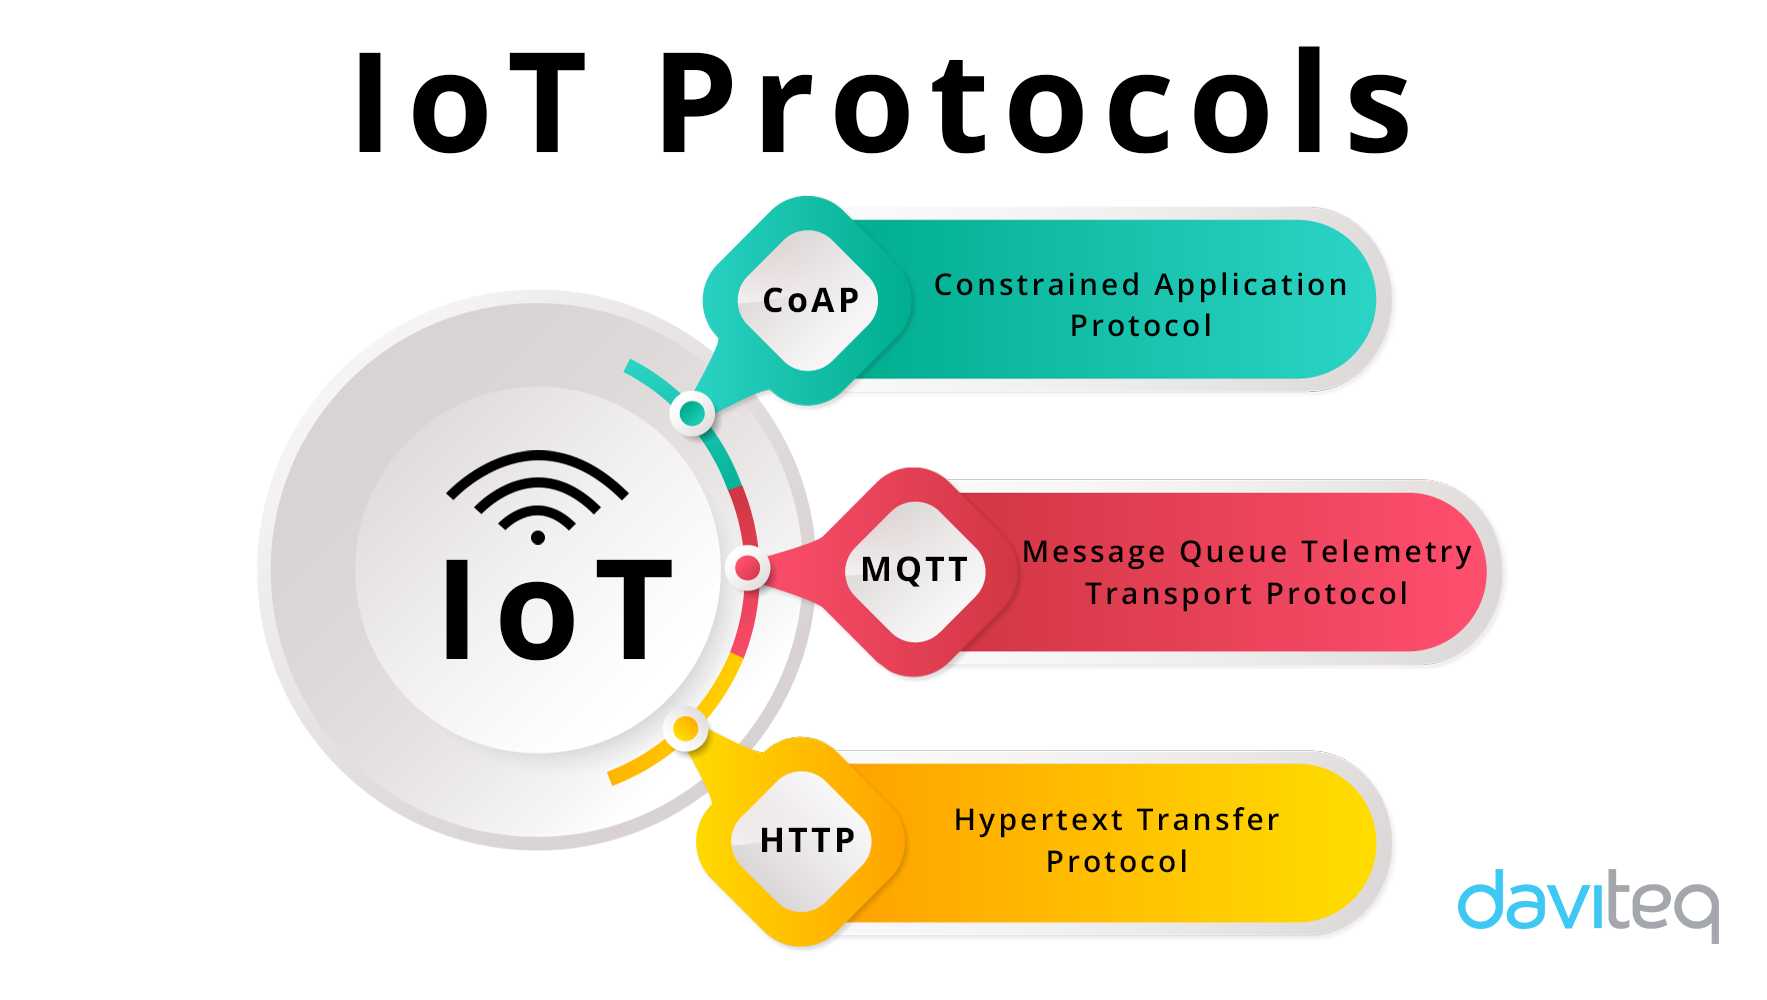
\includegraphics[width=1\textwidth]{coap}
		\caption{Some data protocols for IoT 
			\cite{daviteq}.}
		\label{fig:3layers}
	\end{figure}
		\subsubsection*{MQTT}
The Message Queue Telemetry Transport (MQTT) protocol is a lightweight, open, and simple client-server messaging transport designed for easy implementation. It uses a publish/subscribe message pattern that allows for one-to-many message distribution and is agnostic to the content of the payload\cite{7446846}. The protocol offers three levels of message delivery quality of service, allowing for greater control over network traffic. MQTT is an excellent fit for IoT communication, requiring minimal memory and processing power. Additionally, the protocol is designed for reliability and scalability, with Transport Layer Security enabling security and adaptive connectivity.\cite{particleIoT}

			\subsubsection*{CoAP}
			Constrained Application Protocol (CoAP) is a specialized web transfer protocol designed for Machine-to-Machine (M2M) applications, such as smart city and building automation, with constrained nodes and networks.  CoAP enables resource-constrained devices to communicate with the wider Internet using lightweight packets, thereby reducing network congestion, saving battery power and storage space, and improving the IoT lifecycle.\cite{particleIoT}  CoAP's request and response interaction model between application end points, built-in discovery services, and support for key Web concepts such as URIs and Internet media types make it an ideal protocol for low-power, low-bandwidth network connectivity.  CoAP is designed to integrate seamlessly with HTTP while meeting specialized requirements such as multicast support and simplicity for constrained environments, with a high packet error rate and typical throughput of 10 kbps\cite{7446846}. 
				\subsubsection*{AMQP}
			Advanced Message Queuing Protocol (AMQP) is a protocol designed for corporate messaging, offering a range of features related to messaging such as reliable queuing, flexible routing, and transactions.\cite{8088251}AMQP is a binary protocol that requires a fixed 8-byte header and has a maximum message payload size determined by the broker or programming technology being used. The maximum size of the message payloads is generally small.\cite{7158101}Its use of TCP and TLS/SSL for security makes it a secure and trustworthy protocol for IoT applications\cite{han2015semantic}.Overall, AMQP plays a vital role in enabling communication and coordination among diverse devices in the IoT domain.
		\subsubsection*{HTTP}
		Hyper Text Transport Protocol (HTTP) is widely used as a web messaging protocol for Internet of Things (IoT) applications. Developed jointly by the IETF and W3C, it supports the request/response RESTful web architecture and uses Universal Resource Identifiers (URI) for data exchange\cite{8088251}. Servers send data through URIs, and clients receive data through specific URIs. HTTP is a text-based protocol that does not define the size of header and message payloads, which depends on the web server or programming technology. It uses TCP as the default transport protocol and TLS/SSL for security.Despite now no longer defining QoS, it gives numerous functions together with continual connections, request pipelining,and chunked transfer encoding that make it an ideal protocol for various IoT applications. 
	\subsection{Applications}
	The Internet of Things (IoT) allows us to access clever services in many areas of life. However, because the devices are so varied and interconnected, there can be challenges to overcome. These services include things like transportation, environmental monitoring, healthcare, weather and more.
		\begin{figure}[H]
		\centering
		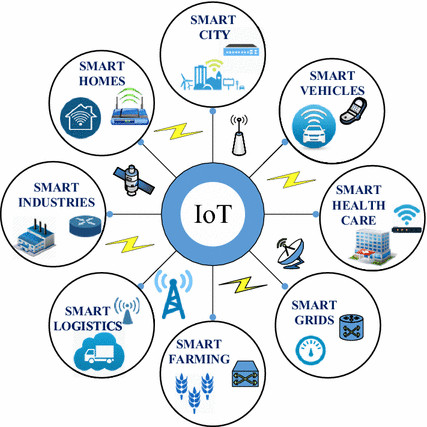
\includegraphics[width=0.6\textwidth]{ss}
		\caption{IoT Applications domains 
			\cite{articleKorea}.}
		\label{fig:iotapp}
	\end{figure}
	\subsubsection*{Smart homes} IoT devices such as smart thermostats, lighting systems, and security cameras can be controlled remotely using a smartphone or voice command, making our homes more comfortable, secure, and energy-efficient. 
	\subsubsection*{Healthcare} IoT devices such as wearables and remote patient monitoring systems can track and transmit health data, allowing doctors and caregivers to monitor patients' health in real-time and provide timely interventions. 
	\subsubsection*{Transportation} IoT-enabled vehicles can communicate with each other and with infrastructure, enabling safer and more efficient transportation, and helping to reduce traffic congestion. 
	\subsubsection*{Agriculture} IoT sensors may be used to reveal soil moisture, temperature, and different environmentalfactors, allowing farmers to optimize crop yields and reduce water and fertilizer usage. 
	\subsubsection*{Manufacturing} IoT-enabled sensors and analytics tools can be used to monitor machine performance and detect maintenance issues, reducing downtime and improving production efficiency. 


			\section{Adjacent technologies}
%\subsection{Definition}

As mentioned in the previous section, the Internet of Things (IoT) has evolved rapidly. technology that connects devices and sensors to the internet, so The success of any IoT project depends on the integration of a range of adjacent technologies,such as  wireless sensor networks, RFID, remote sensing, NFC, video surveillance ... etc \\
These technologies are essential for collecting and processing data from IoT devices, enabling make intelligent decisions and maintain the security and confidentiality of the data generated and transmitted by IoT devices.\\
In this section, we explore the technologies that are closely related to IoT, including Remote Sensing and RFID Technology\\


\subsection{RFID Radio Frequency IDentification Technology}

\subsubsection{Definition}
The RFID (Radio Frequency IDentification) technology also well-known as wireless radio frequency identification,non-contact card and inductive electronic chip or electronic tag . is a wireless (contactless) application known to the traceability, access control and logistics. It became ubiquitous in industry and our daily life (ticketing, payment, passports, car keys, etc.).RFID nowadays is a standardized technology. can offer many advantages, such as unitary, identification, wireless communication, and low cost of tags.\cite{duroc2018rfid}\\

\subsubsection{RFID Systems Structure And Main Components}
%\subsubsection*{*}
RFID systems are generally divided into two layers, physical layer and Information Technology (IT) layer.
The figure below shows the RFID systems architecture and main components:\\
\begin{figure}[h]
	\centering
	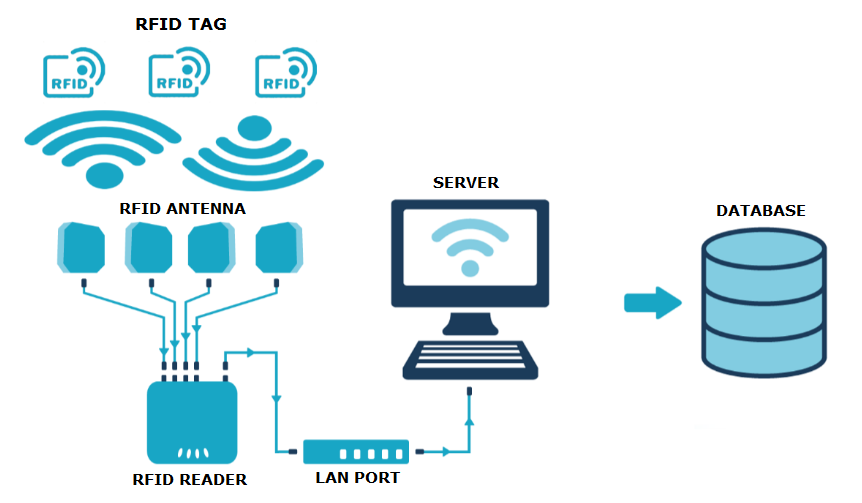
\includegraphics[width=0.8\textwidth,height=0.3\textheight]{images chap1/rfidsys}
	\caption{General RFID system Structure and Main Components }\cite{rfidsys}
\end{figure}

\textbf{physical layer composed of :}
\begin{itemize}
	\item One or more RFID tag or transponder (transmitter/responder), which is consisting of a semi-conductor chip, a contact or contactless wire, and in some cases coupled with a battery.\\
	\item  One or more reader or a read/write gadget(also called an investigator), which is consisting of a RF receiver that typically connected to the reader antenna, and a control hardware module.\\
	\item  A controller connected with PC or a workstation where the data sorted in a database and software controller (middleware).
	\item One or more reader antennas
\end{itemize}
\textbf{Information Technology (IT) layer which consist :}
\begin{itemize}
	\item One or more host computers (or servers) connected to readers (directly or through a network)
	\item Appropriate software (device drivers, filters, middleware, databases, and user applications)
\end{itemize}

% a reader with integrated or external connected antenna, an electronic tag (transponder), and a compute device that hosts a database and an application dependent software package and an application software system. \cite{duroc2018rfid}\\%
%\begin{picture}
%\includegraphics[\textwidth]{rfidsystem}
%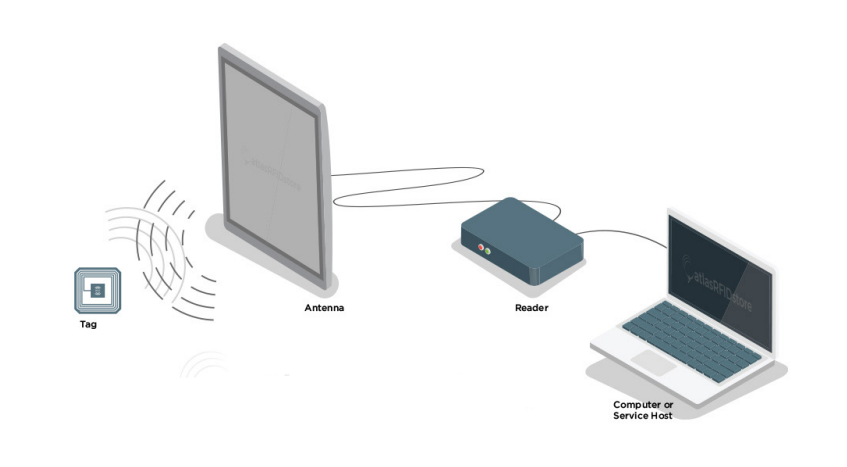
\includegraphics{rfidSystem}
%\end{picture}}
\subsubsection{RFID Work Concept}
Radio frequency identification (RFID) is a type of automatic identification and data capture methods of identifying objects  using radio waves, without the need for physical contact. RFID utilizes radio frequencies to enable two-way communication between a reader and an electronic tag or radio frequency card, allowing for the exchange of data and identification of the object.\cite{li2018flooding}\cite{landaluce2020review}\\

\begin{figure}[h]
	\centering
	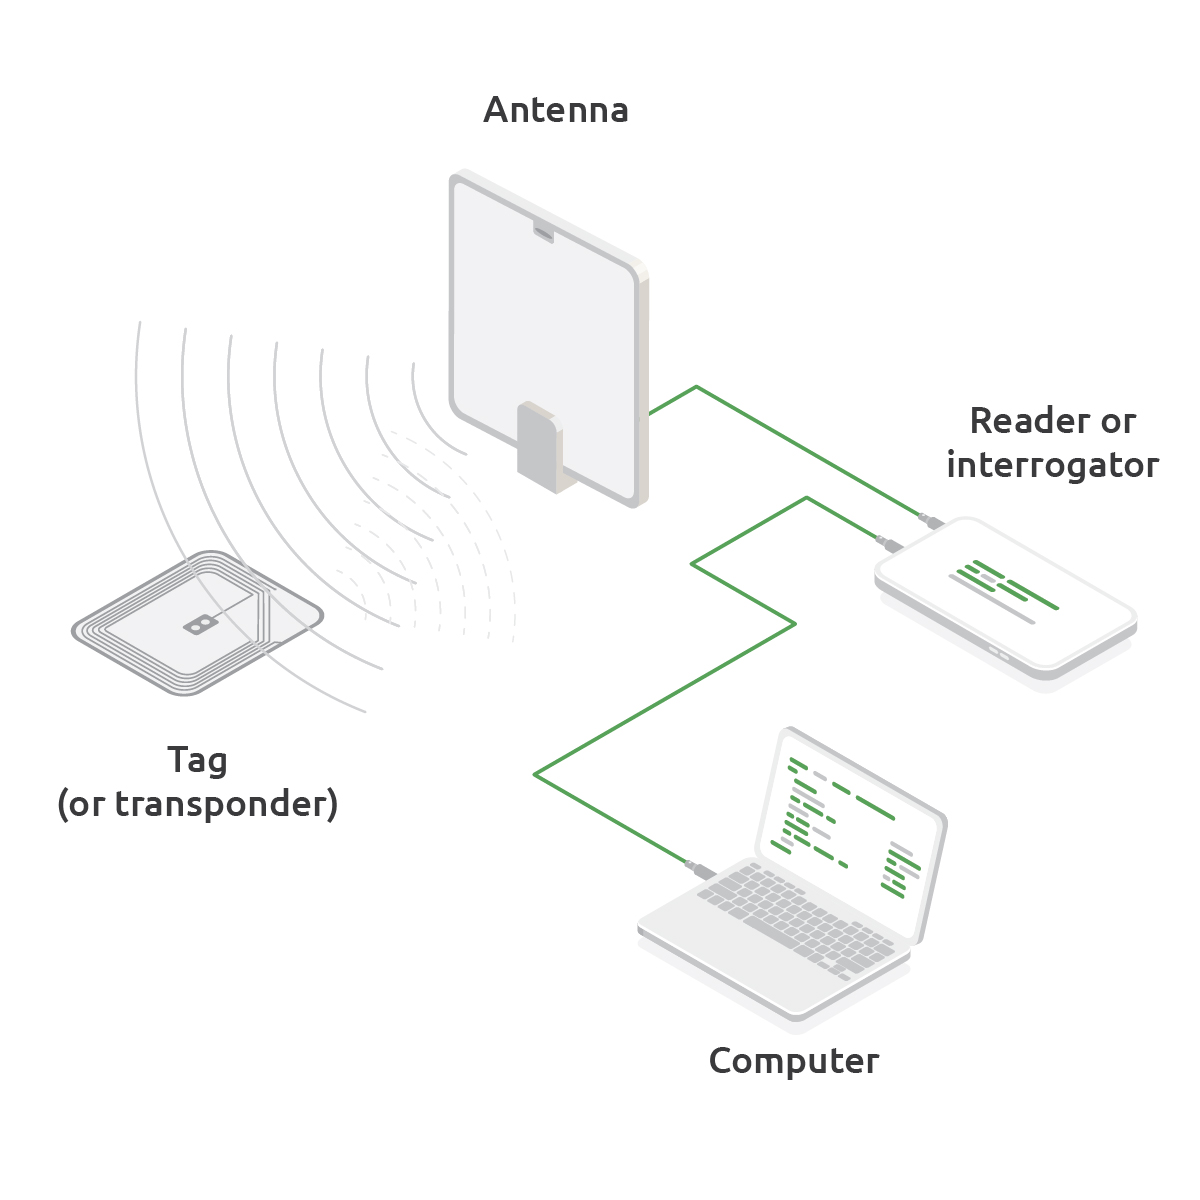
\includegraphics[width=0.8\textwidth,height=0.3\textheight]{images chap1/r}
	\caption{General RFID system Structure and Main Components }\cite{rfidwork}
\end{figure}

This process functions as follows :\cite{li2018flooding}
\begin{itemize}
	\item An RFID system involves attaching a tag to an object, which stores information about the object.
	\item The reader is responsible for powering the tag (just in the passive tag case), identifying it, and reading/writing data from/to the tag.
	\item Additionally, the reader communicates with a database to process information from the tags.
	\item When an object that has an RFID tag on it comes within range of the reader, the reader transmits a radio signal to the tag.
	\item The tag then powers up and sends its information back to the reader, sometimes receiving new information from the reader.
	\item The information is then sent to a database for processing.
	
\end{itemize}
Note : the RFID reader powered only the tags of passive type , the other tag type are powered by other ways.\cite{li2018flooding}\\
Note : since RFID systems use radio waves, the reader's antenna can communicate with the tag without requiring a direct line of sight between them.\cite{li2018flooding}

\subsubsection{RFID System Classification :}
%\subsubsection{RFID System classification}
The RFID systems can be classified based on many parameters such as Power, communication range, data processing, programming, and protocol\cite{duroc2022identification} .the main classification criteria are :\\\textbf{A) according to the RFID tag type (power source of the tags):}\\
RFID tag can be classified according to their power supply source as follows :\\
\begin{itemize}
	
	
	\item \textbf{ Active tags:} These tags have an embedded battery that enables them to emit a signal without needing to be remotely powered. They can achieve reading distances of a few meters and are primarily used for sending large amounts of information over long distances. However, they are more expensive than other systems, require maintenance service, and are less integrated.\cite{chawla2007overview}
	\item \textbf{ Semi-passive tags (also known as semi-active):} These tags are powered by an embedded energy source similar to active tags, but the battery is used to store data between successive communication exchanges rather than sending a signal. Semi-passive tags use backscattering techniques to send back the reader signal and are often used for recording data during goods transporting. They are particularly useful in food traceability and logistic traceability applications that require temperature monitoring and equipment fleet surveillance.
	\item \textbf{ Passive tags:} These are the most commonly used RFID tags due to their low cost, miniature size, and simplicity of architecture. They do not include a battery or RF transceiver like semi-passive and active tags. Instead, they use backscattering techniques to respond to reader commands. A passive tag receives the power needed to operate from the wave incident from the reader. They are compact, simple, and composed of an antenna for communicating with the reader and an electronic chip that integrates memory for storing data to be transmitted.this type of tags are commonly used in stock tracking and the supply chain management applications.
\end{itemize}
\begin{figure}[h]
	\centering
	\includegraphics[width=0.8\textwidth,height=0.25\textheight]{images chap1/rfidpa}
	\caption{RFID tag types }\cite{rfidtype}
\end{figure}

According to the communication distance RFID passive tags can be divided into near-field and far-field. 
For this reason, the data exchange mode between the read/write device and the electronic tag is correspondingly divided into load modulation and backscatter modulation.\cite{rfidpascla}\\

\textbf{B) according to the frequency bands in which the system operate:} \\RFID systems work from Low frequency (LF) to Super (Ultra) High frequency (SHF/UHF),these frequencies have been normalized to avoid interference by other devices of other technologies.\cite{duroc2018rfid} \\
1) Low Frequency\\
2) High Frequency\\
3) Ultra-High Frequency
%4) Microwaves
\begin{figure}[h]
	\centering
	
	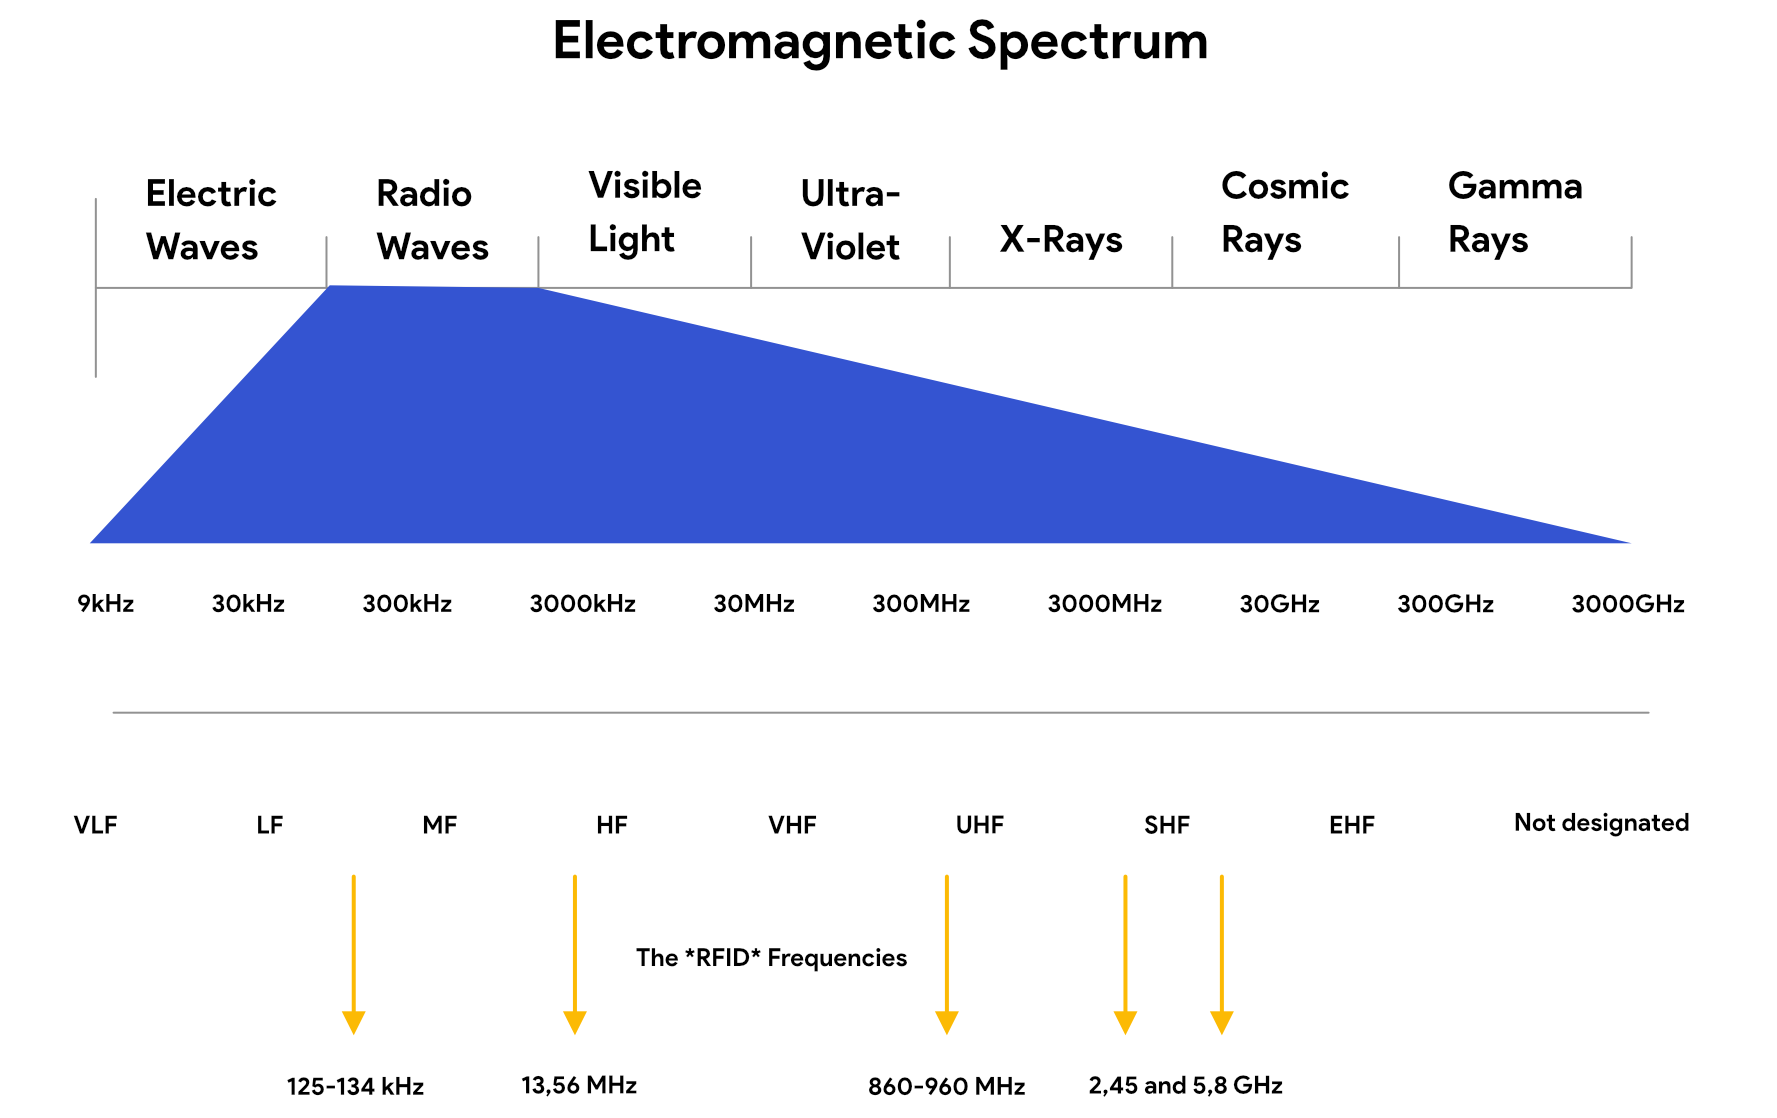
\includegraphics[width=0.9\textwidth ,height=0.3\textheight]{images chap1/rfidfreqs}
	\caption{RFID frequencies in the electromagnetic spectrum}\cite{rfidfreqs}
\end{figure}

we have summarized the most common and frequently used operating frequencies by RFID systems and examples of application in different humanity services in the following table \\
\begin{table}[h]
	
	\centering
	\begin{tabular}{|p{2cm}|p{2cm}|p{1cm}|p{3cm}|p{2.5cm}|p{4cm}|}
		\hline
		frequency &Frequency Range&Read Range&Coupling Type&Existing Standards&Application At The Service Of Humanity\\ \hline
		LF (Passive Tags)&125 khZ 134 KHz &about 0.1 m&Magnetic
		Near field&11784/85, 14223, 18000-2&Smart card, ticketing, access, animal tagging, laundry…\\ \hline
		HF (Passive Tags)&13.56 MHz&about 1 m&Magnetic Near field&18000-3.1, 15693, 14443A, B, C&Small item management, supply chain, anti-theft, library…\\ \hline
		UHF (Passive Tags)&900 MHz 902–928 MHz US
		868–871 MHz Europe
		950–956 MHz Asia&in range 2–20 m&Electromagnetic 
		Far field &EPC C0, C1, C1G2, 18000-6&Transportation vehicle ID, access, security, supply chain, large item management…\\ \hline
		Microwaves (Active Tags)&2.4 GHz  5.8GHz&about 10 m&Electromagnetic Far field&18000-4&Transportation vehicle ID, road toll, access, security, supply chain, large item management…\\ \hline
		
	\end{tabular}
	\caption{RFID Operating Frequencies} 
\end{table}




\subsection{Remote Sensing Technology}
\subsubsection{Definition}
Remote sensing is a technology that allows us to gather information on the Earth's surface and  environment remotely .This can be done using a variety of different sensors, such as cameras; radars, Lidar(Light Detection and Ranging), sonars, lasers,  seismographs or gravimeters. \cite{girard2018processing}\\
\subsubsection{Work Concept}
Remote sensing is a type of data acquisition method typically by using the measurement of electromagnetic radiation emitted or reflected from objects studied in a certain frequency range (infrared, visible, microwaves).\\this is made possible by the fact that the objects studied (plants, houses, water surfaces or air masses) emit or reflect radiation at different wavelengths and intensities depending on their condition. Some remote sensing instruments use sound waves in a similar manner, while others measure variations in magnetic or gravitational fields.\cite{denis2020travaux}

By analyzing the collected data from the sensors, we can gain insights into a wide range of applications, including natural resource management, urban planning, and environmental monitoring like land use, vegetation health, weather patterns, and more.\cite{mather2016classification}
\subsubsection{Types Of Remote Sensing Systems}
Here we mention most common Remote Sensing types: \cite{elachi1988spaceborne}
\begin{itemize}
	\item 	Visual Remote Sensing System (e.g., human visual system)
	\item 	Optical Remote Sensing
	\item 	Infrared Remote Sensing
	\item 	Microwave Remote Sensing
	\item 	Radar Remote Sensing
	\item 	Satellite Remote Sensing
	\item 	Airborne Remote Sensing
	\item 	Acoustic and near-acoustic Remote Sensing
\end{itemize}


\subsubsection{Types Of Sensors In Remote Sensing Systems}
There are two major types of sensors, passive and active, that represent the basic difference between remote sensing systems.\cite{zhou2021potential}\cite{heisig2022predicting}
\begin{itemize}
	\item \textbf{Passive Remote Sensing }\\
	Passive remote sensing records natural radiation from Earth's surface or atmosphere.the Sunlight is the most common source of radiation that is reflected from Earth's surface.\\
	Passive sensors used in remote sensing include radiometers and spectrometers. these sensors operate in different parts of the electromagnetic spectrum,they can measure signals across several spectral bands simultaneously.\\\cite{tong2019trends}
	Images produced from these sensors provide important information about the Earth's surface and atmosphere.those images can help understand physical characteristics of the Earth, such as surface temperature and geological properties.
	An example of a passive sensor is a camera with the flash turned off.
	this method have limitations with cloud cover but provides true-color images.\cite{schroeder2019passive}
	
	\item \textbf{Active Remote Sensing }\\
	Active remote sensing uses active sensors to emit radiation towards a target and then measure the reflected or backscattered radiation.Active sensors include LiDAR, RADAR, scatterometers, and altimeters, which mostly operate in the microwave band of the electromagnetic spectrum.\\
	Active sensors are immune to weather conditions and can function in the dark ,so they can be used in various fields, such as volcanology, forestry, and glaciology.
	As an example Synthetic-Aperture Radar (SAR) technology can penetrate through vegetation to obtain surface layer information.\\
	this method main disadvantage is that the pulse power can interfere with other sources of radiation, requiring additional processing and analysis for clear interpretation.\cite{zhou2021potential}
\end{itemize}
\begin{figure}[h]
	\centering
	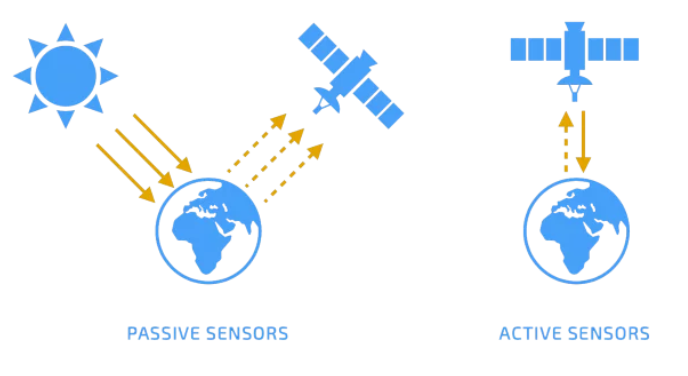
\includegraphics[width=0.7\textwidth ,height=0.3\textheight]{images chap1/rspa}
	\caption{Passive vs Active remote sensing approaches}\cite{rsap}
\end{figure}

\subsubsection{Integration With IoT:}

The integration of remote sensing with IoT technologies can create smart sensing systems that are more efficient and effective. For example, in precision agriculture, remote sensing can be used to collect data on crop health, soil moisture, and other factors, which can be fed into an IoT platform to automatically adjust irrigation or nutrient levels. In disaster management, remote sensing can be used to track the spread of wildfires or floods, while IoT sensors can be used to monitor air quality or track the movement of people and vehicles. In smart cities, remote sensing can be used to monitor traffic patterns, while IoT sensors can be used to monitor air quality, noise levels, and other environmental factors.\cite{ullo2021advances}

\subsubsection{Remote Sensing Applications}
there are a several fields that can integrate remote sensing technology such as :
\begin{itemize}
	\item 	\textbf{Precision agriculture:} Remote sensing can be used in IoT-enabled precision agriculture to monitor crop growth and detect early signs of disease or nutrient deficiency. This can help farmers optimise their harvests and reduce the use of resources. 
	
	\item 	\textbf{Environmental monitoring:} Remote sensing can be used to monitor the health of the environment, including air quality, water quality, and natural disasters. This can be especially helpful in areas subject to pollution or exposed to natural disasters.
	
	\item 	\textbf{Infrastructure monitoring:} Remote sensing can be used to monitor the health and safety of infrastructure such as bridges, dams, and pipelines. This can help identify potential structural issues before they become critical and avoid expensive repairs.
	
	\item 	\textbf{Wildlife conservation:} Remote sensing can be used to monitor wildlife habitats and detect changes in wildlife behavior. It can help environmentalists better understand the needs of animals and take measures to protect them.
	
	\item 	\textbf{Smart cities:} Remote sensing can be used in IoT-enabled smart cities to monitor traffic patterns, energy consumption, and air quality. This enables cities to optimize their resources and enhance the quality of life of their citizens.
	
	\item \textbf{Monitoring crop health and growth:} in agriculture field Remote sensing can be used to track plant growth, detect disease or nutrient deficiencies, and assess overall crop health. This can help farmers make more informed decisions about irrigation, fertilization, and pest control. \cite{schulz2018machine}\cite{chong2017review}\cite{navalgund2007remote}\cite{karthikeyan2020review}
\end{itemize} 
%figure mrygla H hi rasmi
%\begin{figure}[H]
%	\centering
%	\includegraphics[width=0.3\textheight]{rfidpa}
%	\caption{passive and active}
%\end{figure}
		







\section{Artificial Intelligence}

	\subsection{Definition:}
	Artificial intelligence (AI) is a new field of study that involves imitating human thinking in a machine it also refers to the simulation of human intelligence in machines that will be programmed to do tasks that would normally require the need of human intelligence, such as perception, reasoning, learning, and decision-making.\cite{russell2010artificial}.

	\subsection{Applications of Artificial Intelligence:}
		\paragraph{Natural language processing (NLP):}
		NLP is a field of AI that works on enabling machines to understand and interpret  the human language. NLP has many applications that can be used in normal day to day life like: language translation, chat bots, voice assistants and many other various jobs. \cite{christopher1999foundations}.

		\paragraph{Image recognition and computer vision:}
		AI-powered image recognition and computer vision technologies are  fields of technology that use algorithms to enable machines to interpret and understand visual data by classifying objects or patterns within the data and these technologies are used in a wide range of applications, including object detection, facial recognition, medical imaging, and autonomous vehicles. \cite{bishop2006pattern}.

		\paragraph{Predictive Analytic:}
		AI can be used to analyze large datasets and make predictions about future outcomes. Predictive analytic has applications in healthcare, finance, marketing, and many other fields. \cite{shmueli2010explain}.
	
\section{Machine Learning}
	\subsection{Definitions:}
		\paragraph{Definition 1:}
		Machine learning is a form of artificial intelligence that enables computers to learn from data without being programmed explicitly. The primary aim of machine learning is to allow computers to improve their performance on a specific task, such as recognizing images or speech, by analyzing large amounts of data and detecting patterns and trends. This involves the development of algorithms that can learn from the data, make predictions, or decisions based on that data, and create systems that can adapt and enhance their performance over time. The ultimate goal of machine learning is to enable computers to learn and make decisions in a way that simulates human intelligence. \cite{alpaydin2010introduction}.
		\paragraph{Definition 2:}
		Machine learning is a scientific field within artificial intelligence that focuses on the development of algorithms and statistical models to enable computers to act without being programmed explicitly. Its main objective is to teach machines to learn from data and use that knowledge to make decisions or predictions. Machine learning algorithms use statistical techniques to automatically identify patterns and trends in data and use them to make predictions or decisions about new data. This technique has been successfully implemented in numerous domains, such as image and speech recognition, natural language processing, predictive analytic, and self-driving cars, among others. \cite{murphy2012machine}.
		
	\subsection{Features of machine Learning}	
		\paragraph{Automation:}
		Machine learning automates the process of building analytical models. Once trained, a model can be used to make predictions or decisions without human intervention. This means that the system can learn patterns and relationships from data and make decisions based on that learning. The automated nature of machine learning makes it an efficient tool for tasks that require repetitive pattern recognition or analysis. Machine learning models can also be used to automatically detect and diagnose faults in complex systems, such as industrial equipment, by analyzing sensor data. \cite{alpaydin2010introduction}
	
		\paragraph{Adaptivity:}
		Machine learning models can adapt to changing data and learn from new examples. This means that they can improve their accuracy over time and become more effective. As new data becomes available, the model can be updated and retrained to improve its predictions. This adaptability is a key feature of machine learning, as it allows the system to continually learn and evolve to better meet the needs of its users. Machine learning models that can adapt to new data can be used in a wide range of applications, including fraud detection, speech recognition, and autonomous vehicles.  \cite{hastie2009elements}
	
		\paragraph{Generalization:}
		: Generalization is a key aspect of machine learning, which enables models to make predictions on new and unseen data by learning from the training data. The ability to generalize allows machine learning models to identify and apply patterns and relationships in the training data to new, unseen data. This is crucial because models may need to be applied to real-world situations where the training data is unavailable. For example, a machine learning model trained on historical sales data can be used to make predictions about future sales, even if the specific sales data is unknown. The ability to generalize is an important feature of machine learning as it allows models to be utilized in various applications, leading to improved accuracy and efficiency in making predictions and decisions. \cite{bishop2006pattern}
	
		\paragraph{Interactivity: }
		One of the key advantages of machine learning algorithms is their ability to interact with their environment and adapt their behavior in response to feedback. This means that machine learning systems can learn from their users and improve their performance over time. Interactive machine learning systems have a broad range of applications, including virtual assistants, chatbots, and recommendation engines. These systems can learn from user feedback and adjust their recommendations or responses to better satisfy the user's needs. This feature of machine learning is highly beneficial, as it enables the development of intelligent systems that can provide more personalized and accurate recommendations, leading to enhanced user satisfaction. \cite{amershi2014power}
	
		\paragraph{Scalability: }
		Machine learning algorithms are highly scalable, making them suitable for a wide range of applications that involve complex problems and large datasets. This scalability enables machine learning algorithms to be used in areas such as personalized recommendations, fraud detection, and medical diagnosis. The ability to handle large datasets is critical to machine learning as it allows algorithms to learn and make more accurate predictions. The scalability of machine learning models makes them highly versatile and applicable in various fields, including image recognition and natural language processing, where large datasets are crucial for model training and improved performance. \cite{jordan2015machine}
		
		\paragraph{Nonlinearity: }
		Machine learning models are designed to capture complex and often nonlinear relationships between input and output variables, making them highly effective for tasks such as natural language processing and image recognition. Nonlinearity refers to relationships between input and output variables that are not simple or linear, and instead are complex and nonlinear. Machine learning models excel at capturing these complex relationships, which can be used to make highly accurate predictions. For instance, a machine learning model used for image recognition can identify intricate features in an image, such as edges, textures, and colors, to classify it accurately. This feature of machine learning is critical for complex and challenging tasks that require advanced pattern recognition and analysis. \cite{lecun2015deep}
		
		
\section{Deep Learning}
	\subsection{Definitions}
			\paragraph{Definition 1:}
				Deep learning is a field of machine learning that utilizes artificial neural networks with multiple layers to extract complex features and patterns from data. By processing data through a hierarchical system of artificial neurons, deep learning models can identify and learn intricate relationships within the data, making it particularly useful for tasks such as image recognition, speech recognition, and natural language processing \cite{goodfellow2016deep}
			\paragraph{Definition 2:}
			Deep learning is a type of artificial intelligence that trains computers to improve their performance on a task by analyzing and adjusting their internal parameters. By using a layered approach to data processing, each layer of a deep neural network learns to extract progressively more complex features from the data, resulting in more accurate predictions and better generalization to new inputs. Deep learning has demonstrated remarkable success in various fields, such as image and speech recognition, natural language processing, and predictive modeling  \cite{lecun2015deep}
			
	\subsection{Applications :}
			\paragraph{Image Recognition :}
				Deep learning models can be trained to recognize objects in images and classify them into different categories. This technology has been used for facial recognition, object detection, and image segmentation, among other things. One such example is the use of convolutional neural networks (CNNs) for image recognition, which has shown great success in applications like self-driving cars and medical imaging. \cite{krizhevsky2017imagenet}
			
			\paragraph{Natural Language Processing (NLP):}
				Deep learning models can be used for language modeling, sentiment analysis, language translation, and many more NLP applications. For instance, deep learning models like recurrent neural networks (RNNs) have been applied to machine translation tasks, while transformer models such as BERT have been applied to tasks like question answering and sentiment analysis.  \cite{vaswani2017attention}
			\paragraph{Speech Recognition: }
				Deep learning models can be used for speech recognition tasks, including voice recognition, speaker identification, and speech-to-text conversion. Deep neural networks such as long short-term memory (LSTM) networks have been used to build robust speech recognition models. \cite{graves2005framewise}
			
			\paragraph{Autonomous Systems:}
				Deep learning has been applied to develop autonomous systems such as self-driving cars, drones, and robots. Deep reinforcement learning algorithms have been used to enable robots to learn how to perform tasks through trial and error. 	\cite{mnih2015human}
				
\section{Model Learning Methods and CNN}
		\subsection{CNN Definition :}
		A Convolutional Neural Network (CNN) is a type of deep learning model that has proven to be particularly effective in image classification tasks. It works by applying a series of convolutional filters to the input image, which helps to identify and extract meaningful features from the image. These features are then processed through a series of layers, allowing the network to learn increasingly complex representations of the image. The end result is a set of predicted classes or labels that describe the content of the input image. \cite{lecun2015deep}
	%	Reference: LeCun, Y., Bengio, Y., & Hinton, G. (2015). Deep learning. Nature, 521(7553), 436-444.
		
		
		\subsection{how CNN Works:}
		Convolutional Neural Networks (CNNs) are a type of deep learning model used in computer vision tasks, such as image classification, object detection, and segmentation. These models automatically extract important features from input images by applying convolutional filters.
		
		When processing an input image, a CNN uses these filters to detect patterns by sliding over the image and computing dot products between the filter weights and image pixels within the filter's receptive field. Afterward, the resulting feature maps are passed through activation and pooling layers to reduce their spatial resolution and into fully connected layers to classify the image.
		
		During the training process, CNN weights are updated using backpropagation and gradient descent to minimize the difference between the predicted output and the actual output. This allows the model to learn increasingly complex representations of the input image, enabling it to accurately recognize patterns and objects within images. Due to their impressive performance in various computer vision tasks, CNNs are commonly used in the field.
		
		\begin{figure}[h]
			\centering
			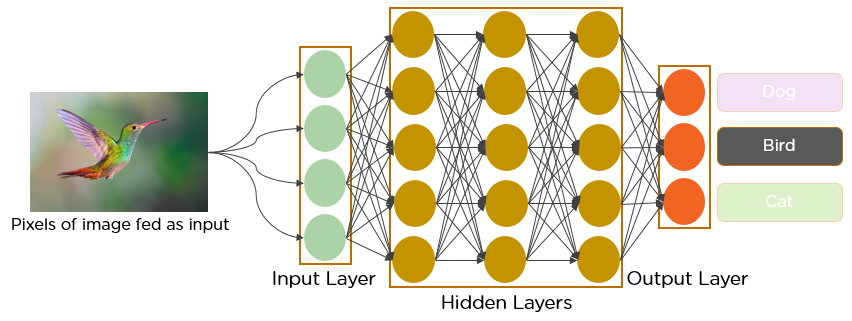
\includegraphics[width=0.8\linewidth]{images chap1/cnnimage.png}
			\caption{How CNN Algorithm Works}
			\label{cnnimage}
		\end{figure}
		
		
		
		\subsection{Learning Methods: }
			\paragraph{Supervised Learning}
			Supervised learning is a machine learning technique where the model is trained on labeled data, enabling it to learn to map input data to output data. This technique is commonly used in tasks such as image classification, speech recognition, and natural language processing. In supervised learning, the labeled data is used to train the model, and the trained model can then make predictions on new, unlabeled data. \cite{alpaydin2010introduction}
		
			\paragraph{Unsupervised Learning}
			Unsupervised learning is a machine learning technique where the model is trained on unlabeled data to find patterns or structure in the data. This technique is commonly used in clustering, dimensionality reduction, and anomaly detection, where the model groups similar data points together based on their similarities or differences. Unlike supervised learning, unsupervised learning does not rely on specific output data to guide the learning process. \cite{goodfellow2016deep}
		%	Goodfellow, I., Bengio, Y., & Courville, A. (2016). Deep Learning (1st ed.). MIT Press.
			\paragraph{Reinforcement Learning}
			Reinforcement learning is a machine learning technique where an agent learns by exploring its environment and receiving feedback. The goal of the agent is to maximize a cumulative reward signal by making decisions that lead to positive outcomes. This approach is commonly used in robotics and game playing, where the agent needs to learn through trial and error. \cite{sutton2018reinforcement}
		%	Sutton, R. S., & Barto, A. G. (2018). Reinforcement Learning: An Introduction (2nd ed.). MIT Press.
			\paragraph{semi-supervised Learning}
			This approach lies between supervised and unsupervised learning, and combines the benefits of both, the model can learn more efficiently and effectively 
			\paragraph{active learning}
			In active learning, the machine learning algorithm selects and queries the user for the most useful data points to label, rather than labeling all data points upfront. This method allows the algorithm to iteratively improve its model's performance, ultimately reducing the amount of labeled data required for training. Active learning is a useful technique in scenarios where labeled data is scarce or expensive to obtain, allowing for more efficient and effective use of resources. \cite{settles2009active}
			%Settles, B. (2009). Active Learning Literature Survey. Computer Sciences Technical Report 1648, University of Wisconsin-Madison.
			\paragraph{transfer learning.}
			Transfer learning is a method of reusing a pre-trained machine learning model's knowledge to solve a different but related problem. The technique involves fine-tuning the pre-trained model using a smaller dataset for the new task. By leveraging the learned features from the original task, the model can achieve better accuracy on the new task than it would without transfer learning.
			\cite{pan2010survey}
			%Pan, S. J., & Yang, Q. (2010). A survey on transfer learning. IEEE Transactions on knowledge and data engineering, 22(10), 1345-1359.
			\begin{figure}[h]
				\centering
				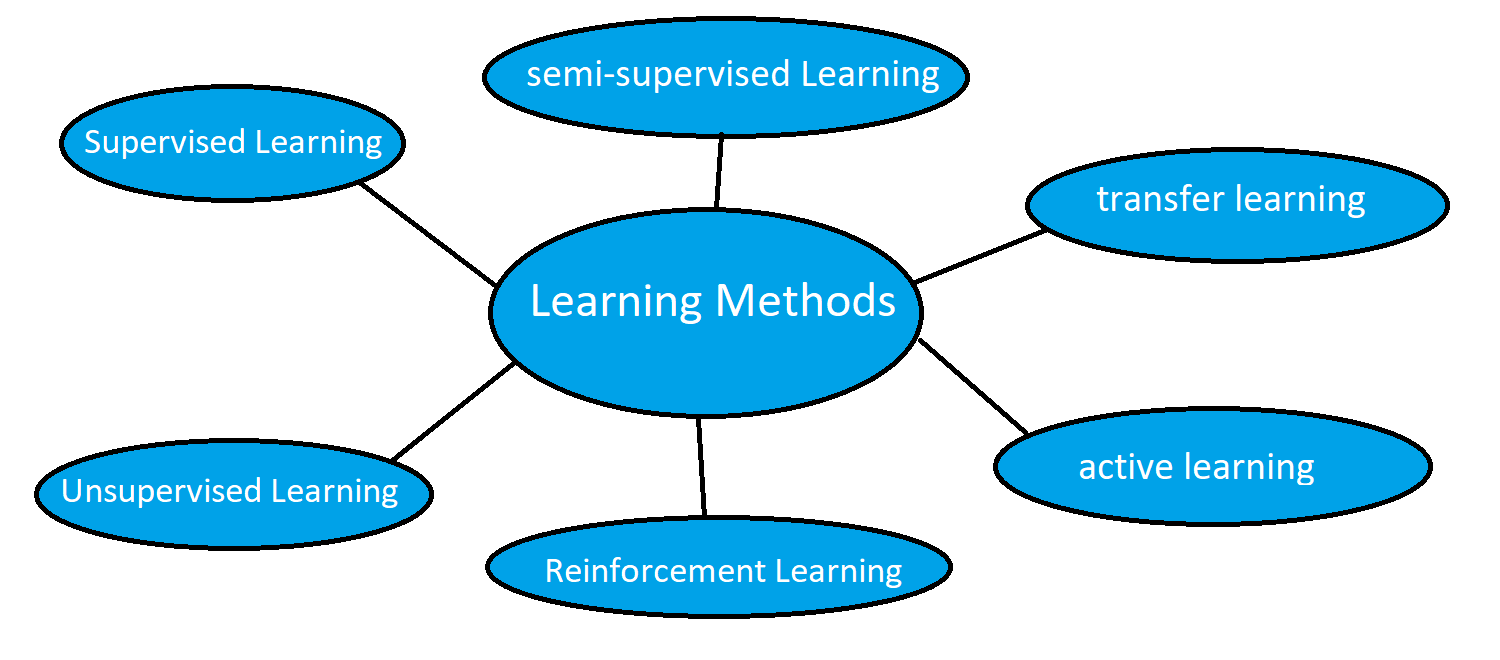
\includegraphics[width=0.8\linewidth]{images chap1/methods.png}
				\caption{Model Learning Methods}
				\label{methods}
			\end{figure}
			
		%	\bibliographystyle{unsrt}
		%	\bibliography{ref}	
		%	\listoffigures


	\bibliography{ref}
	\bibliographystyle{plain}
\end{document}